% SC1005 --- Chapter 1: Number Systems (0->100 ground-up)
\chapter{Number Systems: From Counting to Binary and Hexadecimal}
\label{ch:numbers}

\begin{quote}
\emph{``There are 10 kinds of people: those who understand binary and those who don't.''}
Digital hardware speaks only two voltages. This chapter teaches you to count, compute, and
think fluently in that language, starting from zero---no prior digital background assumed.
\end{quote}

\noindent\fbox{\parbox{\dimexpr\linewidth-2\fboxsep-2\fboxrule}{%
\textbf{From zero: built for absolute beginners.} We assume only school arithmetic.
Every idea is picture $\to$ words $\to$ definition. By the end you will convert,
add, and negate in binary/hex as naturally as in decimal.}}
\vspace{0.4em}

\section*{Learning Outcomes}
After this chapter you will be able to:
\begin{enumerate}[label=(L\arabic*)]
    \item explain positional number systems and weight of each digit position;
    \item convert fluently among decimal, binary, octal, and hexadecimal;
    \item count binary ranges and detect overflow for $n$-bit unsigned numbers;
    \item represent signed integers via sign-magnitude, one's and two's complement;
    \item add, subtract, and reason about overflow in two's complement arithmetic.
\end{enumerate}

% ============================================================
\section{Why Not Decimal Inside a Computer?}
\label{sec:why-binary}
Decimal uses ten symbols; hardware would need ten distinct voltage levels---fragile
against noise. Two levels (\texttt{LOW} $\approx 0$\,V, \texttt{HIGH} $\approx V_{DD}$)
are maximally noise-immune. One binary digit (bit) stores one yes/no choice. Eight bits make a byte,
the standard storage atom. This is why all modern computers are binary at the bottom.

\paragraph{Positional intuition.} In decimal $472 = 4\!\times\!10^2+7\!\times\!10^1+2\!\times\!10^0$.
Replace base $10$ by $2$: each position weighs twice the one to its right. Same rules, smaller base.
The rightmost position is the least-significant bit (LSB), the leftmost the most-significant bit (MSB).

\begin{definition}[Positional representation]
In base (radix) $r$, digits $d_i\in\{0,\dots,r-1\}$ and
\[ N = d_{k-1}r^{k-1}+\cdots+d_1r^1+d_0r^0+\;.\;d_{-1}r^{-1}+\cdots \]
We write $(d_{k-1}\dots d_0.d_{-1}\dots)_r$. Decimal ($r=10$), binary ($r=2$),
octal ($r=8$), hexadecimal ($r=16$, digits $0$--$9,A$--$F$) are the four we use.
\end{definition}

\begin{figure}[h]
\centering
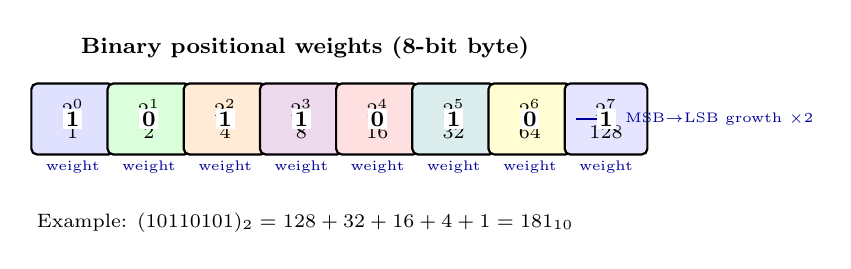
\begin{tikzpicture}[scale=0.82,every node/.style={font=\scriptsize}]
\foreach \i/\w/\col in {0/1/blue!12,1/2/green!14,2/4/orange!16,3/8/violet!14,4/16/red!12,5/32/teal!14,6/64/yellow!18,7/128/blue!10} {
  \node[draw,thick,rounded corners=2pt,fill=\col,minimum width=1.05cm,minimum height=0.9cm,align=center] at (\i*1.18,0.6) {$2^{\i}$\\$\w$};
  \node[font=\tiny,blue!60!black] at (\i*1.18,-0.15) {weight};
}
\node[font=\footnotesize\bfseries] at (3.6,1.7) {Binary positional weights (8-bit byte)};
\draw[->,thick,blue!60!black] (7.8,0.6)--(8.4,0.6) node[right,font=\tiny] {MSB$\to$LSB growth $\times2$};
\node[font=\scriptsize,align=center] at (3.6,-1.0) {Example: $(10110101)_2 = 128+32+16+4+1 = 181_{10}$};
\foreach \i/\b in {0/1,1/0,2/1,3/0,4/1,5/1,6/0,7/1} {
  \node[font=\footnotesize\bfseries,fill=white,inner sep=1pt] at ({(7-\i)*1.18},0.6) {\b};
}
\end{tikzpicture}
\caption{Each binary position weighs a power of two. The rightmost bit (LSB) weighs $1$, next $2$, then $4,8,\dots$.}
\label{fig:binary-weights}
\end{figure}

\section{Conversions}
\label{sec:conversions}
\paragraph{Binary $\to$ decimal:} sum weights of $1$-bits. Example: $(1101)_2 = 8+4+1=13$.

\paragraph{Decimal $\to$ binary:} repeated division by $2$, read remainders bottom-up.
$13\div2=6$ r$1$, $6\div2=3$ r$0$, $3\div2=1$ r$1$, $1\div2=0$ r$1$ $\Rightarrow 1101$.
For fractions, repeated multiply by $2$ and collect integer parts.

\paragraph{Hexadecimal shortcut.} Since $16=2^4$, group bits in fours:
$(1011\,0110)_2 = (B6)_{16}$, and $(3F)_{16}= (0011\,1111)_2$. This is why hex is ubiquitous
in datasheets, addresses, and machine code listings---compact alias for binary.

\begin{figure}[h]
\centering
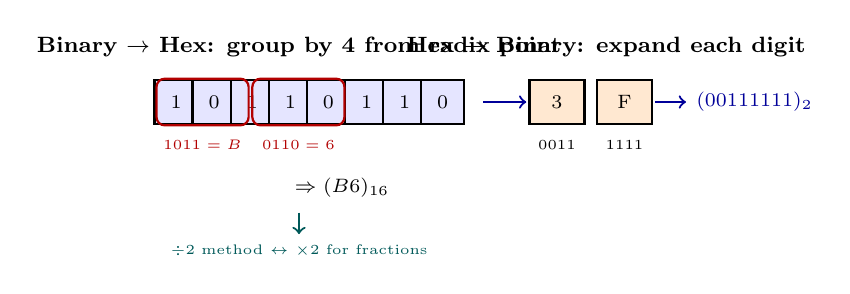
\begin{tikzpicture}[scale=0.78,every node/.style={font=\scriptsize}]
\node[font=\footnotesize\bfseries] at (2.0,1.6) {Binary $\to$ Hex: group by 4 from radix point};
\foreach \i/\b in {0/1,1/0,2/1,3/1,4/0,5/1,6/1,7/0} \node[draw,thick,fill=blue!10,minimum width=0.55cm,minimum height=0.55cm] at (\i*0.62,0.7) {\b};
\draw[thick,red!70!black,rounded corners=3pt] (-0.32,0.32) rectangle (1.18,1.08);
\draw[thick,red!70!black,rounded corners=3pt] (1.24,0.32) rectangle (2.74,1.08);
\node[font=\tiny,red!70!black] at (0.43,0.0) {$1011=B$}; \node[font=\tiny,red!70!black] at (1.99,0.0) {$0110=6$};
\node at (2.7,-0.7) {$\Rightarrow (B6)_{16}$};
\node[font=\footnotesize\bfseries] at (7.0,1.6) {Hex $\to$ Binary: expand each digit};
\foreach \i/\h in {0/3,1/F} { \node[draw,thick,fill=orange!18,minimum width=0.7cm,minimum height=0.55cm] at (6.2+\i*1.1,0.7) {\h}; }
\node[font=\tiny] at (6.2,0.0) {$0011$}; \node[font=\tiny] at (7.3,0.0) {$1111$};
\draw[->,thick,blue!60!black] (5.0,0.7)--(5.7,0.7);
\draw[->,thick,blue!60!black] (7.8,0.7)--(8.3,0.7) node[right] {$(00111111)_2$};
\draw[->,thick,teal!70!black] (2.0,-1.1)--(2.0,-1.45) node[below,font=\tiny] {$\div2$ method $\leftrightarrow$ $\times2$ for fractions};
\end{tikzpicture}
\caption{Binary--hex conversion is lossless grouping by four bits; decimal conversion uses repeated division/multiplication.}
\label{fig:hex-grouping}
\end{figure}

\begin{example}[Conversions]
Convert $(2A.4)_{16}$ to decimal: $2\!\times\!16+10+4/16=42.25$.
Convert $42.25$ to binary: $42=(101010)_2$, $0.25=(.01)_2$, so $101010.01_2$---check hex $2A.4$ matches.
Octal groups by $3$ bits: $(101101)_2=(55)_8$ since $16=2^4$, $8=2^3$.
\end{example}

\section{Unsigned Range and Overflow}
An $n$-bit unsigned integer spans $0$ to $2^n-1$. With $n=8$, $0$--$255$; $n=32$, $0$--$4\,294\,967\,295$.
Adding $1$ to $111\ldots1$ wraps to $00\ldots0$ (overflow / carry out). Hardware signals this with a carry flag.

\begin{figure}[h]
\centering
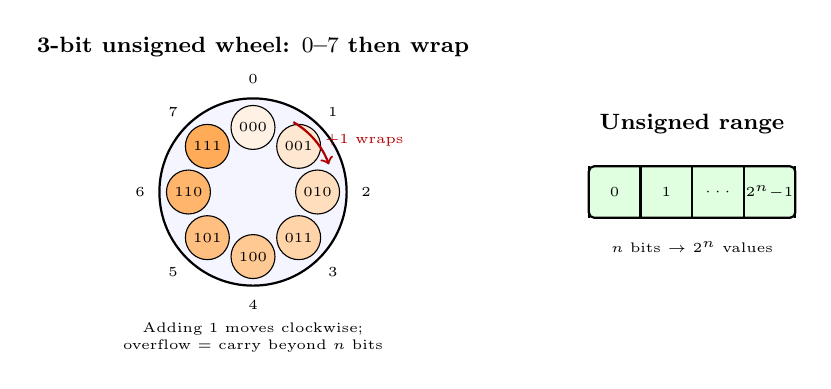
\begin{tikzpicture}[scale=0.82,every node/.style={font=\scriptsize}]
\draw[thick,fill=blue!4] (0,0) circle (1.45);
\foreach \i/\b/\d in {0/000/0,1/001/1,2/010/2,3/011/3,4/100/4,5/101/5,6/110/6,7/111/7} {
  \pgfmathsetmacro{\a}{90-\i*45}
  \node[draw,circle,fill=orange!\the\numexpr 10+\i*8\relax,inner sep=2pt,font=\tiny] at (\a:1.0) {\b};
  \node[font=\tiny] at (\a:1.75) {\d};
}
\draw[->,thick,red!70!black] (60:1.25) arc (60:20:1.25) node[midway,right,font=\tiny] {+1 wraps};
\node[font=\footnotesize\bfseries] at (0,2.25) {3-bit unsigned wheel: $0$--$7$ then wrap};
\node[font=\tiny,align=center] at (0,-2.25) {Adding 1 moves clockwise;\\ overflow = carry beyond $n$ bits};
\begin{scope}[xshift=5.2cm]
\draw[thick,fill=green!12,rounded corners=2pt] (0,0.4) rectangle (3.2,-0.4);
\foreach \x in {0,0.8,1.6,2.4,3.2} \draw[thick] (\x,0.4)--(\x,-0.4);
\node[font=\tiny] at (0.4,0) {$0$}; \node[font=\tiny] at (1.2,0) {$1$}; \node[font=\tiny] at (2.0,0) {$\cdots$}; \node[font=\tiny] at (2.8,0) {$2^n{-}1$};
\node[font=\tiny,align=center] at (1.6,-0.85) {$n$ bits $\to$ $2^n$ values};
\node[font=\footnotesize\bfseries] at (1.6,1.05) {Unsigned range};
\end{scope}
\end{tikzpicture}
\caption{Unsigned $n$-bit numbers live on a wrap-around wheel. The extra carry beyond $n$ bits is the overflow flag.}
\label{fig:number-wheel}
\end{figure}

\section{Signed Numbers and Two's Complement}
Three historical schemes for signed $n$-bit integers:
\begin{itemize}
    \item \textbf{Sign-magnitude:} MSB is sign ($0=+,1=-$), rest is magnitude. Two zeros! Range $-(2^{n-1}-1)$ to $+(2^{n-1}-1)$.
    \item \textbf{One's complement:} Negate by flipping all bits. Also two zeros. Rare today.
    \item \textbf{Two's complement} (universal): Negate by invert+1. One zero, range $-2^{n-1}$ to $2^{n-1}-1$. Addition is same as unsigned---hardware's reason for winning.
\end{itemize}

\begin{definition}[Two's complement]
For $n$ bits, value of bit-vector $b_{n-1}\dots b_0$ is
\[ V = -b_{n-1}2^{\,n-1}+\sum_{i=0}^{n-2} b_i2^i. \]
Negation: $\; -N = \overline{N}+1$ (bitwise NOT plus one). Subtracting $A-B$ is $A+\overline{B}+1$.
\end{definition}

\begin{example}[Two's complement arithmetic]
$n=4$: $+3=0011$, $-3=1101$ (invert $0011\to1100$+1). $3+(-3)=0011+1101=0000$ (carry discarded) correct.
$5+6=0101+0110=1011$ which is $-5$ after wrap---signed overflow since two positives yielded negative.
$4$-bit range is $-8$ to $+7$; $1011$ as signed is $-5$, as unsigned is $11$.
\end{example}

\begin{theorem}[Overflow rule]
Signed overflow in two's complement addition occurs iff carry into sign bit $\neq$ carry out of sign bit,
equivalently: adding two same-sign numbers yields opposite sign. Unsigned overflow is simply carry out $=1$.
\end{theorem}

\section{Binary Codes and Arithmetic Preview}
Not all bit patterns are numbers. \textbf{BCD} encodes each decimal digit in $4$ bits (wasteful but decimal-exact, used in calculators).
\textbf{Gray code} changes one bit per step---ideal for rotary encoders and Karnaugh maps (no glitch).
\textbf{ASCII/Unicode} map bit patterns to characters; $(41)_{16}$ = `A', $(30)_{16}$ = `0'.
Binary addition is column-wise with carries, exactly like decimal but base $2$: $1+1=0$ carry $1$, $1+1+1=1$ carry $1$.


\section{Fractions, Floating-Point Preview, and Binary Arithmetic}
Binary fractions mirror decimal: $(0.101)_2 = 1/2+1/8=0.625$. Not every decimal fraction terminates in binary
($0.1_{10}=0.00011\overline{0011}_2$ recurring), which is why floating-point rounding matters---preview for
computer arithmetic courses. Binary addition is column-wise:
\begin{center}
\begin{tabular}{rccccc}
 & 1 & 0 & 1 & 1 \\ % 11
+& 0 & 1 & 1 & 0 \\ % 6
\hline
carry &1&1&0&0\\
result&1&0&0&0&1 % 17 - need 5 bits? Actually 11+6=17=10001
\end{tabular}
\end{center}
Carry propagates left; the extra carry beyond $n$ bits is exactly the unsigned overflow flag $C$.
Subtraction via two's complement: $A-B=A+\bar B+1$, so one adder does both operations with an invert-and-carry-in control.

\begin{example}[Overflow table]
$n=4$ signed: $7+1=0111+0001=1000$ ($-8$) overflow; $-8-1=1000+1111=0111$ ($+7$) overflow.
Unsigned, $15+1=1111+0001=0000$ carry $1$---correct modulo $2^4$ wrap.
\end{example}

% ============================================================

% ============================================================
\section{Chapter Notes}
Positional notation dates to Hindu-Arabic mathematics; binary championed by Leibniz (1703).
Two's complement emerged with early stored-program machines (EDSAC, 1949) for its single-adder economy.
Hex became standard with the IBM System/360 (1964) to print 32-bit words compactly.

% ============================================================
\section{Fixed-Point vs.\ Floating Preview}
Fixed-point binary $(b_{k-1}\dots b_0.b_{-1}\dots b_{-m})_2$ has uniform step $2^{-m}$ and range $\approx2^k$.
More bits after the point = finer resolution; more before = larger range. For large dynamic range,
floating-point (sign $\times$ mantissa $\times2^{\text{exponent}}$) trades uniform precision for wide range---full
treatment in computer arithmetic courses. Key takeaway: not all reals are representable; rounding error is inevitable
and must be bounded (e.g.\ unit in last place, ULP).

% ============================================================

\section{Exercises}
\label{sec:ch01-exercises}
\begin{enumerate}[label=E1.\arabic*, leftmargin=*, itemsep=0.8em]
    \item \textbf{Conversions.} Convert $(101101.101)_2$ to decimal, hex, and octal. Convert $(3A7)_{16}$ and $(275)_8$ to binary. Show steps (division/multiplication).
    \item \textbf{Two's complement.} For $n=8$, give binary for $+73$, $-73$, $-128$, $+127$. Compute $73+(-98)$ in binary and flag signed and unsigned overflow.
    \item \textbf{Range and wrap.} An $n=5$ unsigned counter increments by $1$ from $0$. After how many increments does it first read $0$ again? Repeat for signed two's complement starting at $+15$ and incrementing.
    \item \textbf{Hex dump reading.} A memory dump shows \texttt{DE AD BE EF}. Write as binary, as four unsigned bytes decimal, and as two 16-bit big-endian unsigned values. What about little-endian?
    \item \textbf{Gray vs.\ binary.} Construct 3-bit Gray code, show adjacent words differ by one bit, and explain why a 2-bit transition $011\to100$ in binary could briefly read $111$ on skewed wires.
\end{enumerate}
% End of Chapter 1
